Over the last decade, the concept of uncertainty quantification (UQ) has become central for a wide range of application areas \cite{xiu2010}. The primary target of UQ is characterization of the output of the systems that exhibit non-deterministic behavior due to the presence of uncertainties of some kind \cite{eldred2009}. A multiprocessor platform is a prominent example of such a system, wherein the variability originates from, \eg, the semiconductor manufacturing process and operating environment. In particular, the uncertainty impacts power and, consequently, temperature, which are among the main concerns of embedded systems designs. As an example, consider a quad-core architecture subjected to uncertainty in the leakage current\footnote{The experimantal setup is thoroughly explained in \sref{experimental-results}.} and assume, for now, that the parameters, which affect leakage, have nominal values. We can then simulate the system to observe the corresponding temperature. The result, labeled as ``Nominal'', is depicted in \fref{motivation-curve} where, for clarity reasons, only two curves, \ie, two processors, are preserved (the two bottom blue lines). It can be seen that the temperature is always below $70^{\circ}$C. Now, we let mild deviations occur and run the simulation once again. The result is the ``Mild'' curves in \fref{motivation-curve} (the two middle orange lines); the maximal temperature is $80^{\circ}$C. Finally, we repeat the experiment for severe deviations of the leakage parameters and obtain the last two curves in \fref{motivation-curve} labeled as ``Severe'' (the two top green lines); the temperature already approaches $110^{\circ}$C. Therefore, if the nominal parameters were exclusively taken into account, the system might not be designed for such high temperatures; in other words, the chip might have already been burnt. Consequently, the uncertainty has to be addressed if robustness is concerned. At the same time, one can observe that the majority of the literature, which involves system-level power-temperature analysis (PTA), ignores these important aspects, \eg, \cite{rao2009, rai2011, thiele2011, ukhov2012}; therefore, the reliability of the corresponding results is questionable in practice.

To overcome the limitations of the deterministic PTA, a number of stochastic PTA techniques have been recently introduced. A solely power-targeted but temperature-aware solution is proposed in \cite{chandra2010}, which employs Monte Carlo (MC) simulations to account for process and environmental variations of multiprocessor systems. A learning-based approach is presented in \cite{juan2011} to estimate the maximal temperature under the steady-state condition and variability of the leakage current. Leakage is also considered in \cite{juan2012}, where a statistical model of the steady-state temperature based on Gaussian distributions is derived. None of the aforementioned techniques attempts to perform the stochastic \emph{transient} PTA and to compute the evolving-in-time probability distribution of temperature. However, such transient curves are of practical importance. First of all, certain procedures cannot be undertaken without the knowledge of time-dependent temperature variations, \eg, the reliability optimization based on the thermal-cycling fatigue \cite{ukhov2012}. Secondly, when the steady-state assumption, considered, \eg, in \cite{juan2011, juan2012}, fails---which is often the case since power profiles are not invariant in reality, and the thermal time constant of on-chip components is small enough to make temperature follow the power pattern---the steady-state PTA is of little use, and the transient counterpart is to be performed. Furthermore, the frequently made assumption that power and/or temperature follow \apriori\ known probability distributions---for instance, Gaussian and log-normal distributions are popular choices, as in \cite{juan2012, srivastava2010}---is debatable due to (a) the strict nonlinearities between the process parameters, power, and temperature; (b) the nonlinear interdependency of temperature and the leakage power \cite{liu2007}. To illustrate this, we performed $10^4$ simulations of the example in \fref{motivation-curve}, where the distribution of the leakage parameters was taken from the literature (discussed in \sref{illustrative-example}), and employed kernel density estimation to construct probability density functions of the four processors at the middle of the time span shown in \fref{motivation-curve}. The distributions are depicted in \fref{motivation-pdf}, which are neigher Gaussian nor log-normal. To confirm this, we applied the Jarque-Bera test \cite{juan2012} of normality the original data as well as to the data processed by the Box-Cox transformation \cite{juan2012}. In both cases, the null hypothesis, \ie, the data are from a Gaussian distribution, was rejected at the level of significance 5\%. To conclude, the present models of uncertainty and the stochastic PTA techniques for multiprocessor system design are restricted in use due to one or several of the following traits: based on MC simulations (potentially slow as we shall discuss shortly) \cite{chandra2010}, limited to power analysis \cite{chandra2010}, limited to the assumption of the constant steady-state temperature \cite{juan2011, juan2012}, exclusive focus on the maximal temperature \cite{juan2011}, \apriori\ chosen distributions of power and temperature \cite{juan2012, srivastava2010}. Consequently, there is a lack of flexible stochastic PTA techniques, which we aim to fulfill.

\begin{figure}
  \centering

  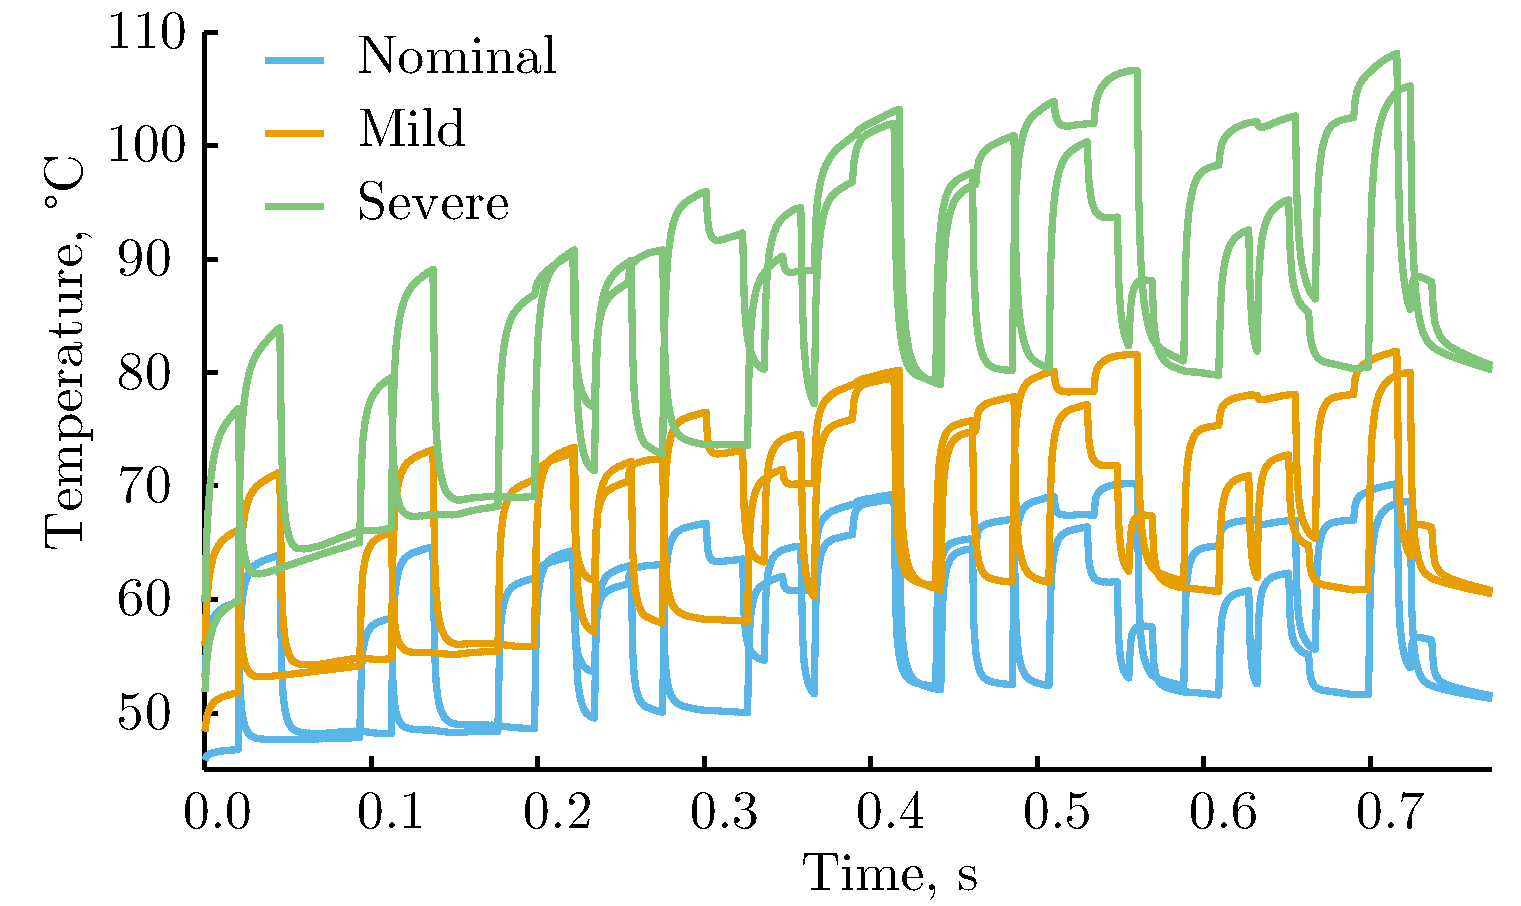
\includegraphics[width=0.8\linewidth]{include/assets/motivation-curve.pdf}
  \caption{Temperature fluctuation due to process variation.}
  \flabel{motivation-curve}

  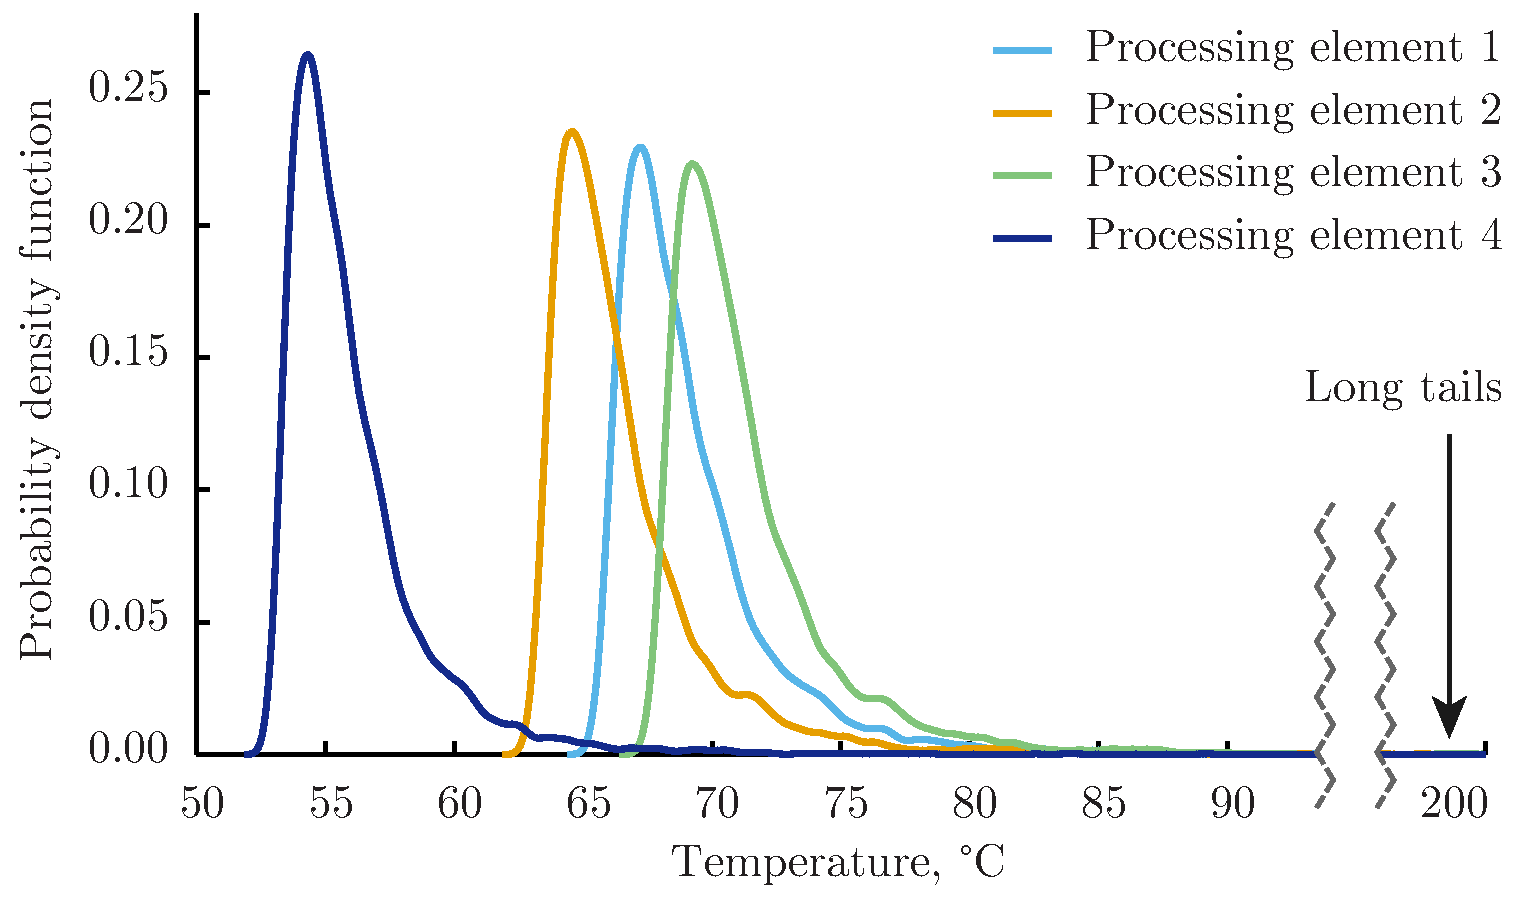
\includegraphics[width=0.8\linewidth]{include/assets/motivation-pdf.pdf}
  \caption{Empirical probability density function.}
  \flabel{motivation-pdf}
  \vspace{-2.05em}
\end{figure}

A straightforward approach, which is mentioned earlier in the context of \cite{chandra2010}, to analyze a stochastic system is the MC sampling coupled with a deterministic simulator. The major problem with the MC sampling is the low rate of convergence, \eg, the mean value converges as $\mcsamples^{-\ifrac{1}{2}}$ where $\mcsamples$ is the number of samples \cite{xiu2010, maitre2010}. This means that, in order to get an additional decimal point of accuracy, one has to obtain hundred times more samples, and each of such samples is a complete realization of the whole system. Therefore, MC-based methods are typically slow and often infeasible since the number of needed simulations can be extremely large in order to obtain reliable estimates \cite{diaz-emparanza2002}.

Attractive alternatives to the MC sampling are spectral methods \cite{xiu2010, maitre2010, ghanem1991} featuring much faster convergence properties. One of such method is applied in this paper, namely, the generalized polynomial chaos (PC), which is the current state of the art in numerical analysis of stochastic systems \cite{xiu2010}. The popularity of PC is dictated by its applicability to a wide range of UQ problems and, more importantly, by its ability to construct easy-to-analyze representations of system responses to stochastic inputs \cite{eldred2009}. In other words, given a computationally intensive model subjected to uncertainty, PC produces a light surrogate, which possesses a number of advantageous, from the post-processing perspective, features. To name few, the cumulative distribution function (\cdf) and probability density function (\pdf) \cite{durrett2010} can be estimated by sampling a trivial polynomial expression, which should be contrasted with the direct, expensive MC sampling of the original model; the expected value, variance, and other moments of higher orders can be determined analytically without any sampling. PC is commonly accompanied by another spectral method called the Karhunen-Lo\`{e}ve (KL) expansion, which we also utilize. KL typically acts at the preprocessing stage and parametrizes the model in terms of a finite---and often much smaller yet sufficient---set of uncorrelated random variables (\rvs); the technique is especially useful if the presence of uncertainty is characterized by a stochastic process, \ie, an infinite collection of \rvs. As it has already been mentioned, such spectral methods are widespread. For instance, in \cite{shen2009}, PC based on Hermite polynomials is employed to estimate the full-chip leakage; the KL expansion is used in \cite{bhardwaj2006} to calculate the leakage current of electrical circuits; an analysis of the voltage response of power grids is carried out in \cite{ghanta2006}, where the PC and KL expansions are jointly utilized.

The contribution of this paper is in the following: we develop, for the first time, a framework for UQ of transient power and temperature variations of multiprocessor systems that depend on a number of uncertain parameters. The framework is flexible in modeling diverse probability distributions of the parameters, which are specified by the user, and there are no assumptions on the distributions of the resulting power and temperature traces as these distributions are unlikely to be known \apriori. Furthermore, the proposed technique is capable of capturing arbitrary joint effects of the uncertain parameters on the system since the parameters are introduced into the model as a ``black'' box, which is also defined by the user. Based a nominal dynamic power profile, our technique produces the corresponding stochastic power and temperature profiles given as polynomials of \rvs; the expressions are straightforward to be further analyzed. The framework is illustrated on one of the most important parameters affected by process variation: the subthreshold leakage current. Note, however, that our approach is not bounded to any particular source of variability and, apart from the process-related variations, can be applied to other uncertainties such as those that are due to environment.

\begin{figure*}
  \vspace{-1.0em}
  \centering
  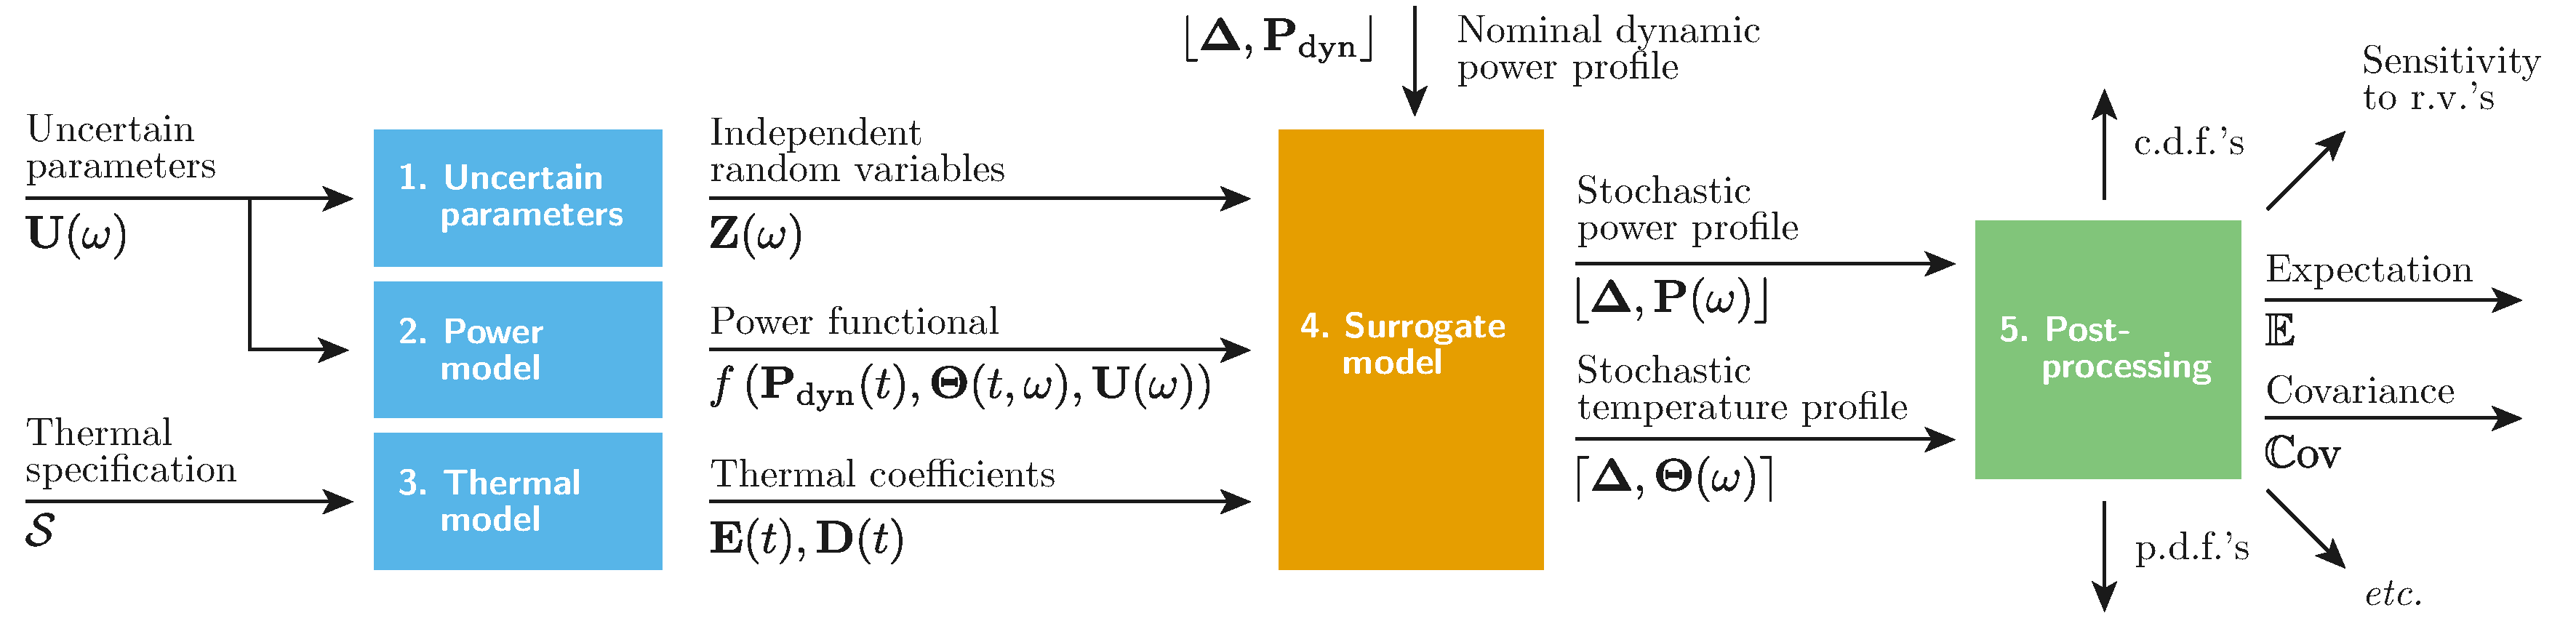
\includegraphics[width=1\textwidth]{include/assets/algorithm.pdf}
  \vspace{-1.0em}
  \caption{The structure of the proposed framework.}
  \flabel{algorithm}
  \vspace{-1.0em}
\end{figure*}

The reminder of the paper is organized as follows. In \sref{preliminaries}, we introduce the architecture model, which we shall consider, and formulate the objective of our study. The proposed framework is presented in \sref{proposed-framework}, wherein a rather general description is given. A particular application of our technique is discussed in \sref{illustrative-example}, and the corresponding results are compared with an MC-based approach in \sref{experimental-results}. \sref{conclusion} concludes the paper. The work also contains supplementary materials with in-depth discussions on certain aspects of our approach; the materials reside in the appendix and are referenced to by the capital letter ``S'', \eg, \aref{thermal-model}.
